
\subsection{Risk-based Resilience Quantification using Multi-criteria Decision Making}
\subsubsection{Prior work in Resilience Metric and Their Limitations}

In literature, multiple articles have sought to define the resilience metrics and have proposed several methods to solve the resilience planning problem. The existing metrics for resilience can be broadly categorized as: a) attribute-based metrics that identify power system attributes such as robustness, resourcefulness, adaptivity, recoverability, and situational awareness~\cite{kandaperumal2020resilience} and b) performance-based metrics that describes the system's ability to maintain supply (i.e., the system's availability~\cite{cai2018availability}) and often measured using the conceptual resilience curve~\cite{panteli2017power}. 
Different resilience indicators that are widely used in literature are based on the optimal repair time of critical components~\cite{wen2020resilience}, energy not served after an extreme event~\cite{espinoza2017seismic}, total critical loads supplied during the aftermath of a disaster~\cite{poudel2018critical}, and  in terms of infrastructure recovery~\cite{umunnakwe2021quantitative}. 
The resilience of power distribution systems is dependent on several factors such as network configuration, available resources and controls, and several other smart grids features such as distributed energy resources (DERs), smart switches, intentional islanding, and self-healing. Towards this goal, references~\cite{7728107, chanda2016defining} introduce the use of multi-criteria decision-making (MCDM) methods to quantify resilience by taking different topological parameters based on graph theory.

Despite these existing approaches no formal resilience metric is universally accepted. The existing metrics to quantify power distribution system resilience pose one or more limitations including: (1) they are post-event measures and mostly evaluated for a single event~\cite{gao2016resilience, poudel2018critical, wen2020resilience} ; (2) they do not specifically measure the impacts of HILP events on system performance (kW loss, critical assets without power, total outage duration)~\cite{7728107, chanda2016defining}; (3) they do not provide additional flexibility to system operators to prioritize one investment decision over the other to evaluate the system resilience~\cite{8767980}. 

\subsubsection{Proposed Risk-based Resilience Metric}
In contrary to reliability assessment, events with higher impact and lower probability are considered for resilience analysis~\cite{panteli2015grid}. Thus, this dissertation proposes a probabilistic approach to calculate the resilience metric that captures both the system attributes as well as its response to a given extreme event. Prior to this work, our group proposed a framework to evaluate the resilience of power distribution systems using conditional value-at-risk as a risk measure~\cite{poudel2019risk}. The specific contributions are listed below:

\begin{enumerate}
    \item \textit{Multi-criteria Risk-based Resilience Metric:} A novel risk-based resilience metric that considers a comprehensive power system resilience definition. The proposed metric takes multiple resilience-driven parameters -- availability, robustness, brittleness, resistance, and resourcefulness to holistically evaluate the power distribution system resilience based on these parameters. 
    \item \textit{Comprehensive Simulation Framework for Resilience Quantification:} A simulation-based approach that allows system operators to evaluate different mitigating actions. The proposed framework provides additional flexibility to prioritize one investment decision over the others to enhance the system's resilience; The operators can come up with economic investment decisions without compromising the resilience of the system.   
\end{enumerate}

\subsubsection{Resilience-driven Parameters and Metrics: Definition}

\begin{figure}[!ht!]
    \centering
    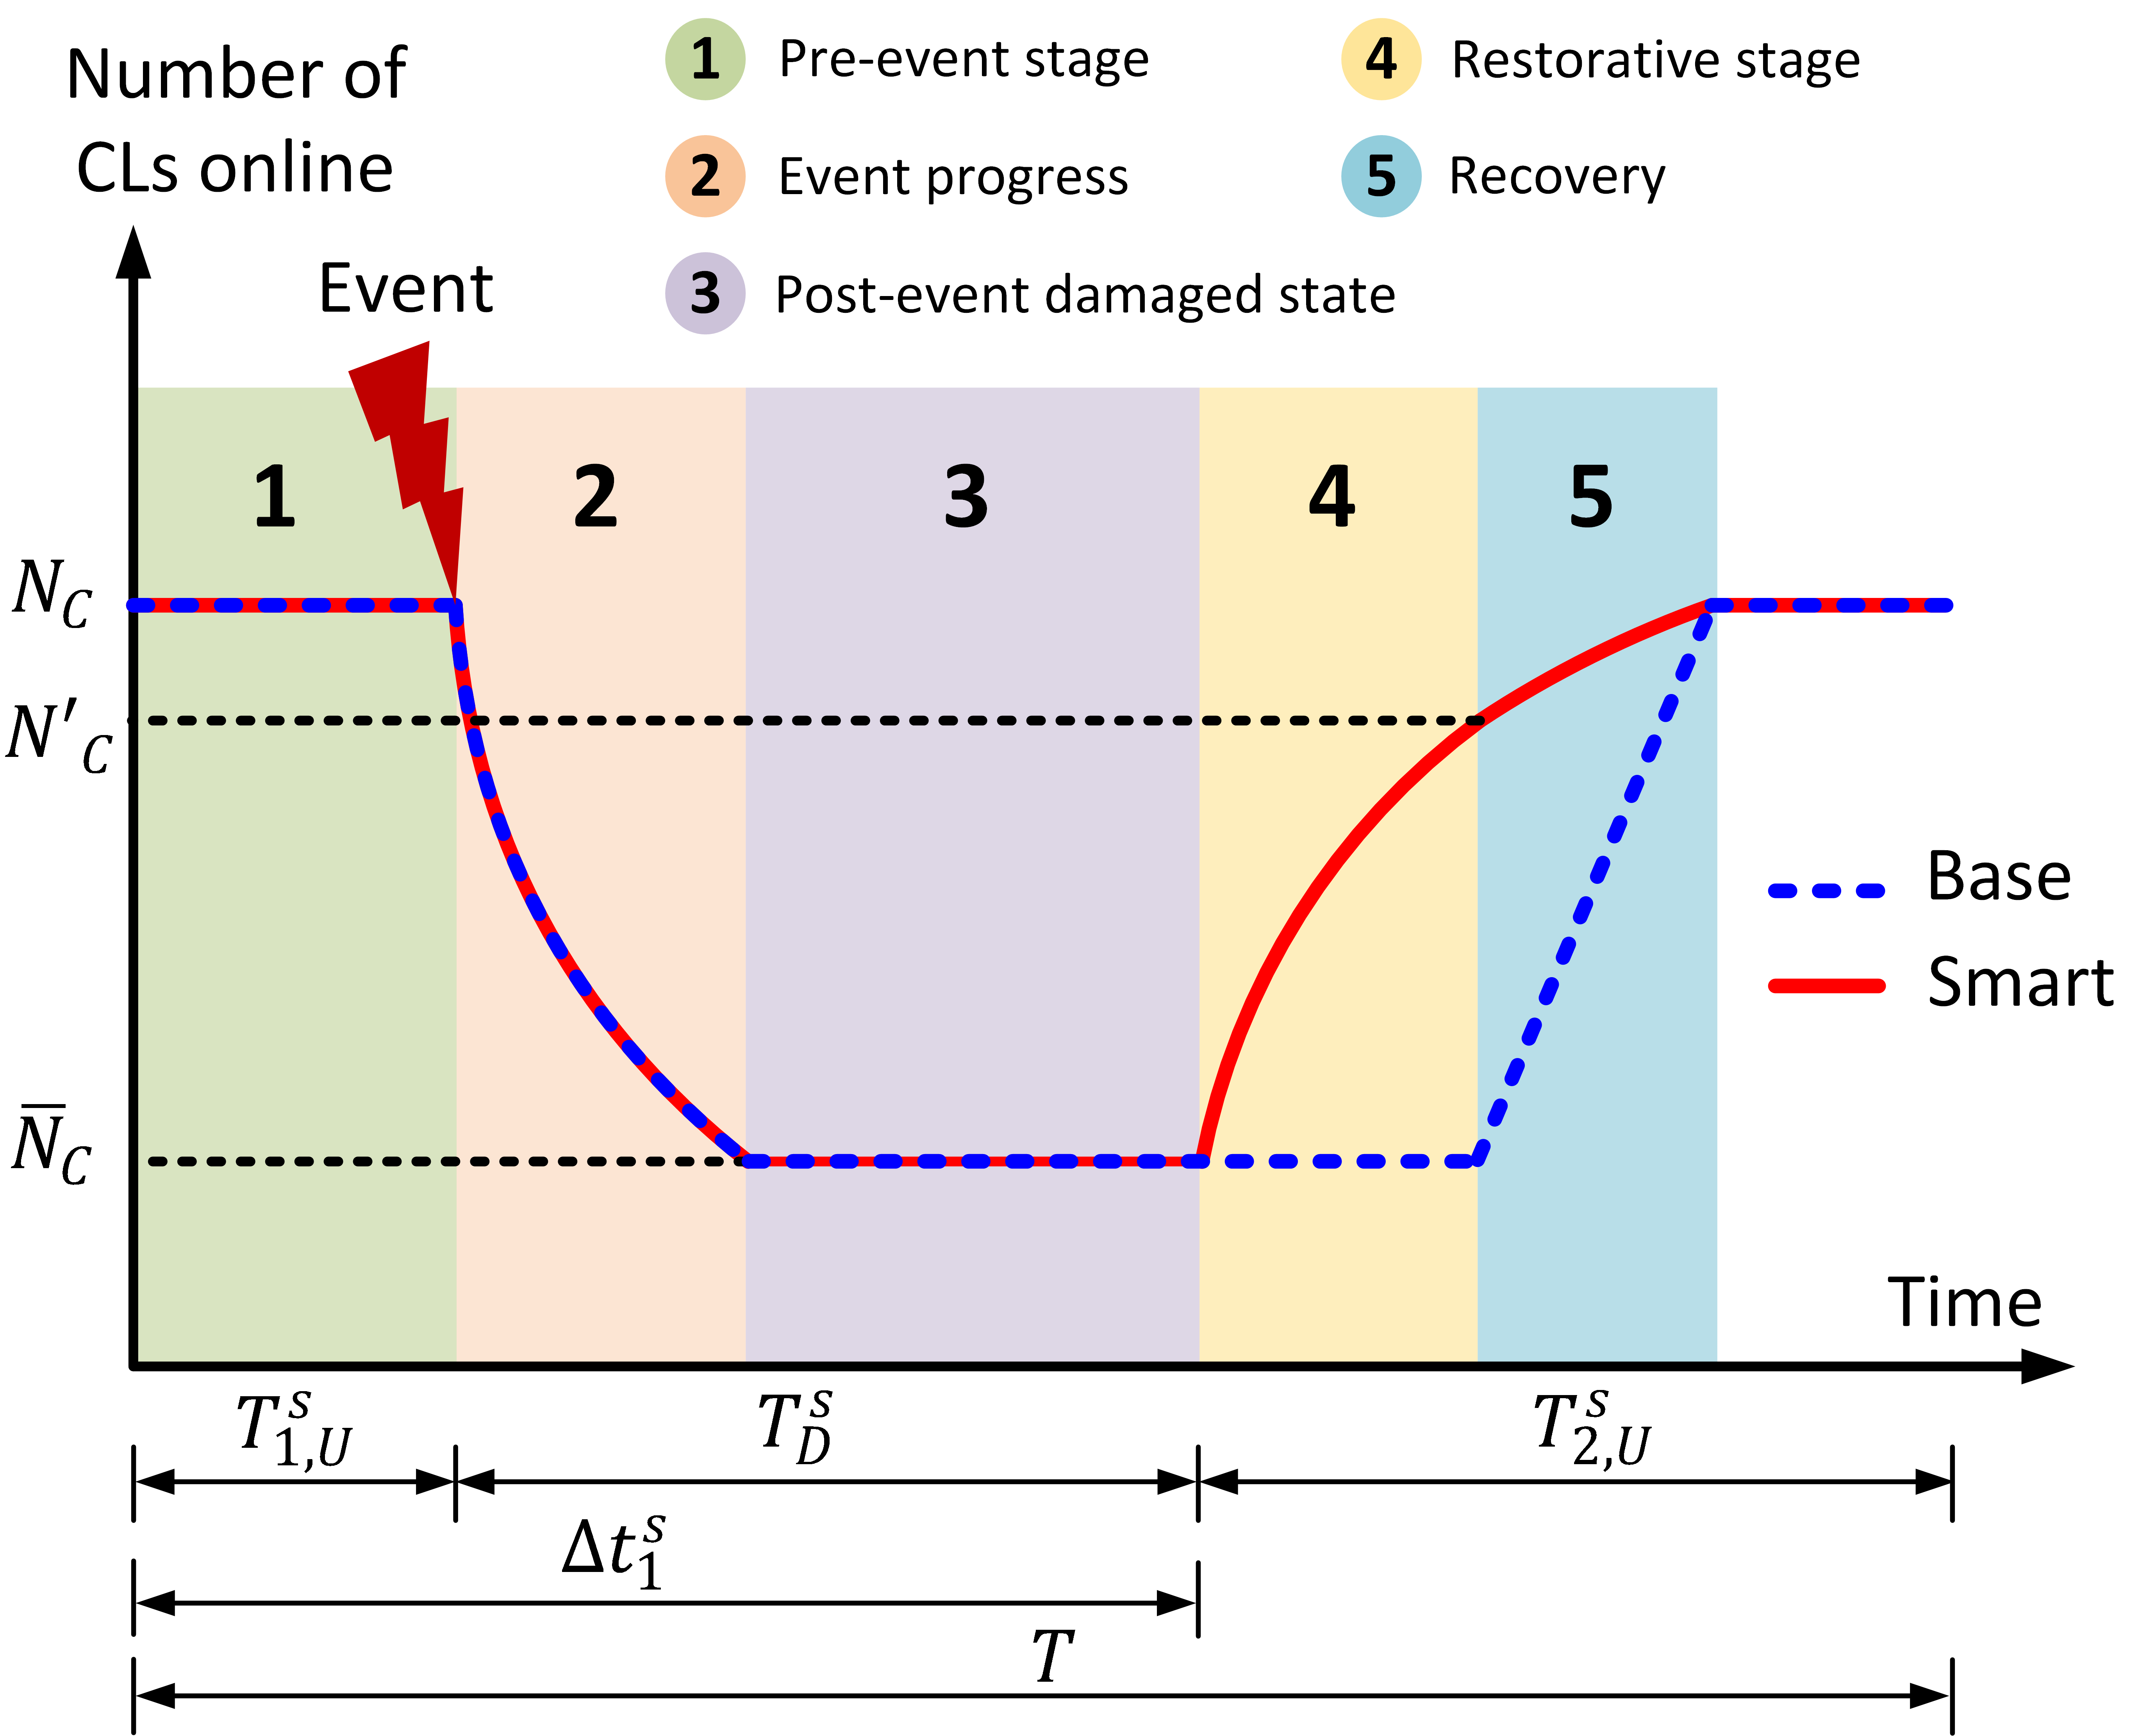
\includegraphics[width=0.65\textwidth]{figures/resilience_curve.png}
    \caption{Typical resilience assessment curve based on the number of weighted CL online. The time variables on the $x$-axis refer to the smart network~\cite{2016}.}
    \label{fig:resilience_curve}
\end{figure}

\paragraph{Resilience Parameters:}\label{par:resilience_parameter}

Fig.~\ref{fig:resilience_curve} shows a typical resilience assessment curve in which the $x$-axis represents time whereas the $y$-axis represents the number of weighted CLs online. Let $N_C$ be the total number of CLs that are online at a particular instance of time. The time in which all of the CLs remain online to the time an event occurs is denoted by $T_{1,U}$ and represented by phase 1. In this work, $T_{1,U}$ is considered the same for all CLs. The event occurs at the end of $T_{1,U}$ and sustains for a certain time. The time of event progress depends on the nature and intensity of the event and is denoted by phase 2 of the resilience assessment curve. Some CLs get disconnected due to the severity of the event. $\Bar{N}_C$ be the number of CLs that remain online after an event occurs. Phase 3 denotes the time for damage assessment. Smart networks have smart devices and damage assessment tools that can decrease the damage assessment time significantly. The CLs get disconnected when an event occurs until the point when repair or restoration starts. This is the downtime for CL and is denoted by $T_D$. $\Delta t_1$ is the period from the initial time to the time when repair/restoration begins. For the base case, the repair does not start until the recovery state, phase 5, whereas for the smart network DGs and remote-controlled switches (RCSs) can assist in load restoration, phase 4. At the point of repair/restoration, some of the CLs become online again and remain online for a time $T_{2,U}$. Let $N'_C$ be the number of CLs that are online after the load restoration phase. The total up and downtime of CL for the entire duration is represented by $T=T_{1, U} + T_D + T_{2,U}$. 

In this work, we only consider phases 1 through 4 for quantifying the resilience metric. We will discuss a few parameters that help us define the resilience of a distribution grid as referred to the critical loads and phases described in Fig.~\ref{fig:resilience_curve}. A detailed explanation of these parameters are given in~\cite{2016} while some of them are modified as necessary for this work.

\paragraph*{Availability:}

Let $i = 1, 2, ... ,N_C$ be the CLs connected in a system, $T_U^i = T_{1,U}^i + T_{2,U}^i$ be the time period when a CL $i$ is connected to system (up time), and $T_D^i$ be the time period when $i$ is disconnected from the system (down time) due to an extreme event. Hence, availability refers to the fraction of time when $i$ is online and is defined as:
\vspace{-3pt}
\begin{equation} \small
    \mathcal{R}_\psi = \frac{\sum_{i=1}^{N_C} T_U^i}{\sum_{i=1}^{N_C} (T_U^i + T_D^i)}
    \label{eq:availability}
\end{equation}

\noindent
Here, $T_U^i$ and $T_D^i$ for each $i$ depends on the type of network. For smart network, some disconnected CLs are restored in phase 4 which increases the overall availability of the system. Here, the choice of $N_C$ is problem specific and can represent a single customer as well as a particular feeder~\cite{2016}.   

\paragraph*{Robustness:}

Let $n_0$ be the number of CLs that are disconnected from the system at a given time. Then the outage incidence, $\theta$ is defined as:
\vspace{-5pt}
\begin{equation} \small
    \theta = \frac{n_0}{N_C}
    \label{eq:max_incidence}
\end{equation}

\noindent
If $N_C - \Bar{N}_C$ be the maximum number of CLs disconnected from the system and $\theta_{max}$ is the maximum outage incidence for a given time, then robustness is defined as:
\vspace{-3pt}
\begin{equation} \small
    \mathcal{R}_\beta = 1 - \theta_{max} = 1 - \frac{N_C - \Bar{N}_C}{N_C} = \frac{\Bar{N}_C}{N_C}
    \label{eq:robustness}
\end{equation}

% Robustness of a system is entirely dependent on the nature of the event and infrastructure of the system. Hence, this attribute is independent of the type of network --- Base or Smart.

\paragraph*{Brittleness:}

Let $D$ be the percentage of infrastructure damage in the system. For simplicity, we only consider distribution lines as infrastructures in this work. Brittleness is the level of disruption that occurred in the system with respect to damage. For instance, if the damage of a single distribution line affects the entire system then the system is highly brittle. The brittleness of a system with $N_C$ critical loads is defined as:
\vspace{-3pt}
\begin{equation} \small
    \mathcal{R}_\gamma = 100 \times \frac{\theta_{max}}{D}
    \label{eq:brittleness}
\end{equation}

\paragraph*{Resistance:}

According to~\cite{2016}, a system has higher resistance if it can withstand extreme events better and can operate the loads for a longer period before getting disconnected. With this notion, a resistant system should have better physical infrastructures, proper damage assessment methods, and situational awareness in case of extreme events. Furthermore, the resistance is also dependent on the nature of the extreme event. Here, $\sigma$ is the measure of an extreme event and is obtained as described in~\cite{2016}. Based on the measure of the event and time before which the repair and restoration begins, the resistance of a system is given by:
\vspace{-3pt}
\begin{equation} \small
    \mathcal{R}_\xi = \frac{\sigma \sum_{i=1}^{N_C} T_{1,U}^i}{\theta_{max} N_C \Delta t_1}
    \label{eq:resistance}
\end{equation}

\paragraph*{Resourcefulness:}

Let $N_{SW}$ be the number of tie-line switches, $N_S$ be the number of generating sources, and $N_P$ be the number of simple paths from each of the sources to CLs after an event has occurred in a network. Then the available resources are useful only if their existence is meaningful in system restoration. Thus, resourcefulness is defined as:
\vspace{-3pt}
\begin{equation} \small
    \mathcal{R}_\delta = \frac{N_P}{(N_{SW} + N_S) \times N_C}
    \label{eq:resourcefulness}
\end{equation}

For the base network, the only available source is the substation so $N_{S} = 1$ for the base case. For the smart network, $N_{S}$ increases as the number of DG increases. However, the resourcefulness decreases if those DGs are not utilized in network restoration after the event has occurred which is ensured by $N_C$. Thus, resourcefulness can be useful for planning the placement and number of DGs to enhance system resilience.

\paragraph{Risk Metrics:}

As discussed in~\cite{poudel2019risk}, we use $CVaR$ as a risk measure for each of the parameters. $VaR$ is defined as the specific threshold $\zeta$, such that with a specified probability of $\alpha$ $VaR$ does not exceed $\zeta$. On the other hand, $CVaR$ is the expected value of the distribution that exceeds $VaR$. Both of these metrics depend on the value of $\alpha$ and are commonly represented as $VaR_\alpha$ and $CVaR_\alpha$. If $p(I)$ be the probability distribution of a random weather event $I$ then the cumulative probability distribution that the parameter $\mathcal{R}$ will not exceed $\zeta$ when impacted by $I$ is given by:
\vspace{-5pt}
\begin{equation} \small
    \Psi (\zeta) = \int_{\mathcal{R}(I)\leq \zeta }^{} p(I) dI
\end{equation}

\noindent Thus, $VaR_\alpha$ and $CVaR_\alpha$ are then defined by:
\vspace{-5pt}
\begin{equation} \small
    VaR_\alpha (\zeta) = \inf\{\zeta \in \mathbb{R}:\psi(\zeta)\geq \alpha\}
    \label{eq:var}
\end{equation}
\vspace{-10pt}
\begin{equation} \small
    CVaR_{\alpha} (\zeta) = (1-\alpha)^{-1}\int_{\mathcal{R}(I)\geq VaR_{\alpha} }^{} \mathcal{R}(I)\ p(I)\ dI
    \label{eq:cvar}
\end{equation}

\noindent $CVaR_\alpha$ represents the value of parameter for the extreme $(1-\alpha)\%$ of impacts. It is also to be noted that the distribution of parameters below and above the specified threshold $\zeta$ represent the complete distribution of extreme events with a probability of $\alpha$ and $1-\alpha$ respectively.

\paragraph{Multi-criteria Decision Making using Choquet Integral:}
When it is essential to include multiple criteria in a decision making process then a single attribute or performance-based analysis do not accurately justify the decision. The Choquet Integral is an effective method for the MCDM problem~\cite{choquet} and is well suited for our framework.

If $\mu$ denote the fuzzy measure on $\Gamma$ then the discrete Choquet integral of a function $f:\Gamma\rightarrow\mathbb{R}^+$ with respect to $\mu$ is defined as~\cite{choquet}:
\vspace{-3pt}
\begin{equation} \small
    \mathcal{C}_\mu(f) := \sum_{i=1}^{n}(f(i)-f(i-1))\mu(\{\mathcal{R}_1, \mathcal{R}_2, .... , \mathcal{R}_n\})
    \label{eq:choquet}
\end{equation}

\noindent
where $f(.)$ are arranged in ascending order of its magnitude and is the $CVaR_\alpha$ of the parameters calculated using~(\ref{eq:cvar}), $\mu({\mathcal{R}})=\eta_\mathcal{R}$ is defined as the Shapely value which accounts for the behavioral analysis of any fuzzy measures, and $f(0) = 0$. More detail information on the Shapely value analysis and fuzzy measures is provided in~\cite{2006}. Choquet integral gives the overall score of alternative decisions in problem involving multiple parameters for each decision.

\subsubsection{Probabilistic Event and Impact Assessment}
Fig.~\ref{fig:ysys} shows the overall framework to quantify the system resilience using a stochastic simulation-based approach and is described in detail below. It is to be noted that the smart network contains DG-based restoration and RCS that can improve the damage assessment and restoration phase to enhance the overall resilience of the system.   
\begin{figure*}[t]
    \centering
    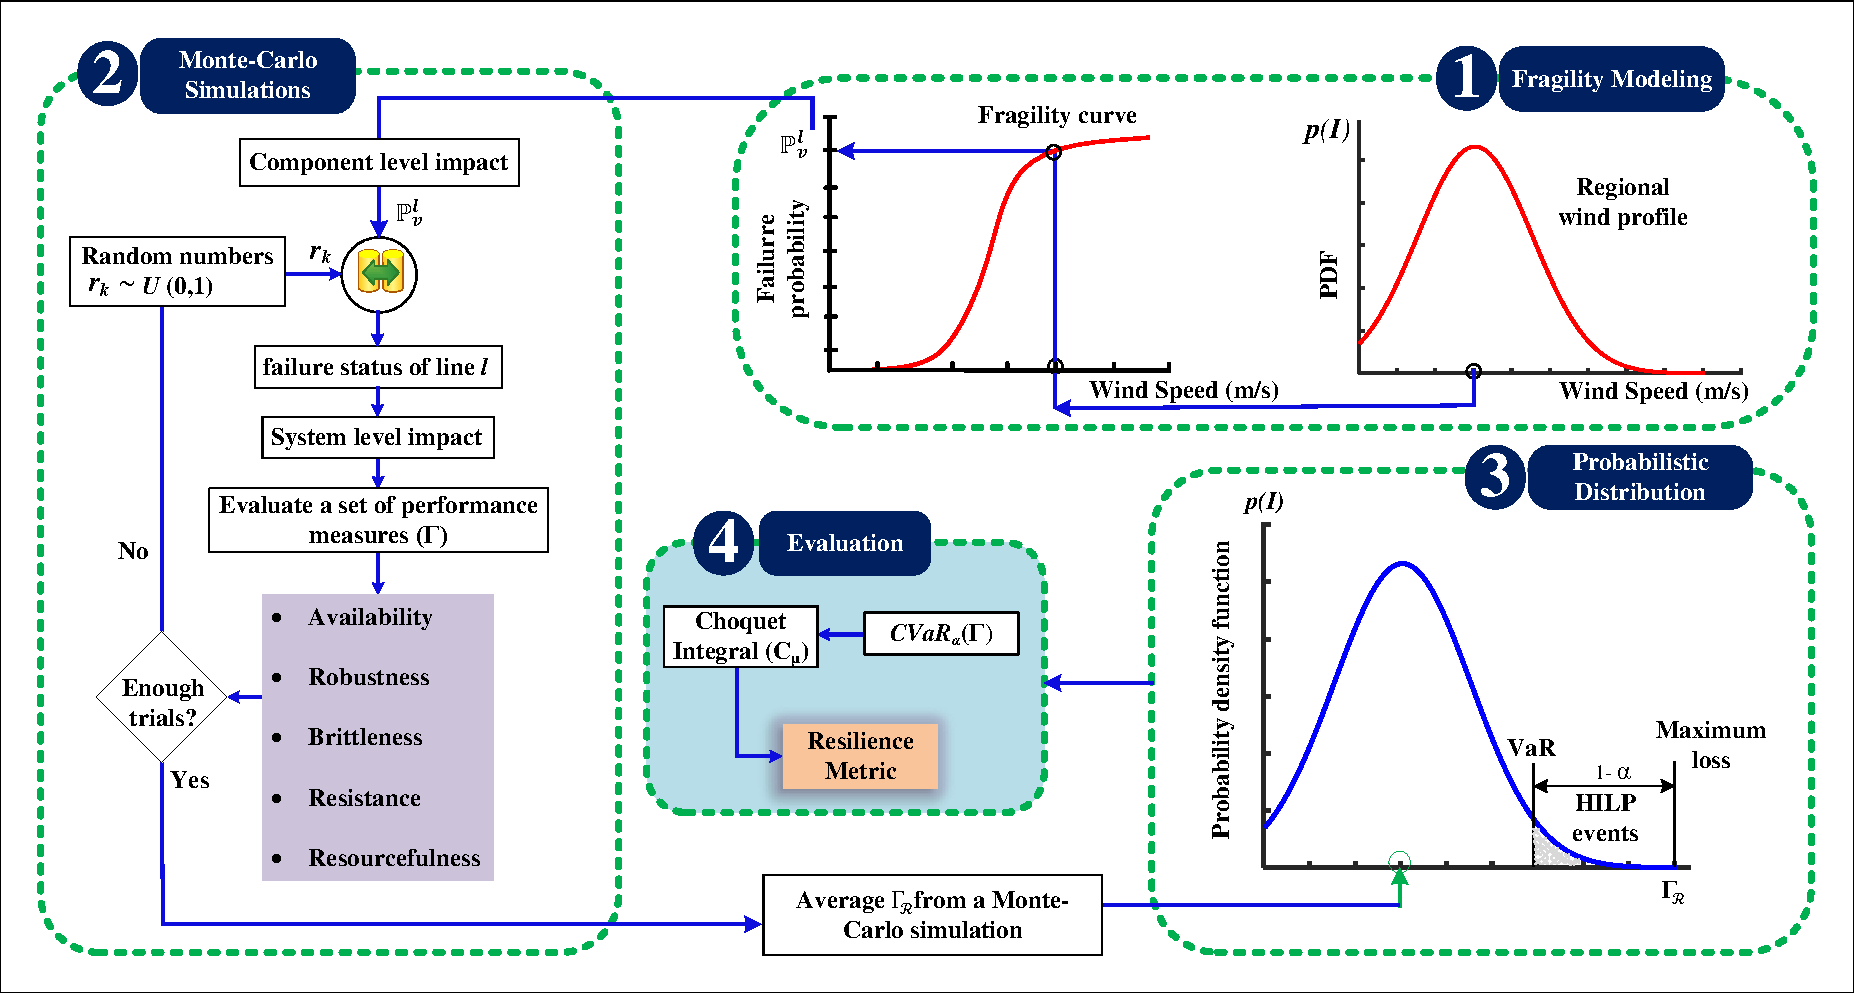
\includegraphics[width=0.9\textwidth,trim={0.5cm 0.25cm 0.35cm 0.5cm}, clip] {figures/MCS.pdf}
    \vspace{-0.2 cm}
    \caption{Simulation-based framework for resilience metric computation; Fragility modeling feeds the failure probability to Monte-Carlo simulation. Monte-Carlo simulation calculates the average value of a performance measure for a given event. $CVaR_\alpha$ is then calculated using the pdf of a given extreme event case.}
    \label{fig:ysys}
    \vspace{-0.3 cm}
\end{figure*}

The extreme wind event and its impact is characterized using its probability distribution and line fragility model. The fragility model of any distribution line gives the outage probability of the line subjected to a particular wind speed and can be represented as:
\vspace{-5pt}
\begin{equation} \small 
\begin{aligned}
&\mathbb{P}_v^l= \begin{dcases}\mathbb{F}_n^l & v < v_{cri} \\
\mathbb{P}^l (v)  & v_{cri} \leq v < v_{col} \\
1 & v \geq v_{col} 
\end{dcases} \\
\end{aligned}
\label{eq:outage}
\vspace{-3pt}
\end{equation}
where $\mathbb{F}_n^l$ is the failure rate of line $l$ in normal weather condition, $\mathbb{P}^l (v)$ is the failure probability of line $l$ as a function of $v$, $v_{cri}$ is the critical wind speed at which line $l$ experiences failure, and $v_{col}$ is the wind speed threshold beyond which line $l$ is guaranteed to fail. Since the process of identifying an event and its impact is purely stochastic, Monte-Carlo simulations are conducted to evaluate the probabilistic impacts of the event on the power distribution grid. The approach is generic as each event is simulated for several trials. The fragility models provide the failure probability of any distribution lines. With the increase in wind intensity, the failure probability increases accordingly. Monte-Carlo simulations help us identify the number of lines being failed in each trial, and resilience-driven parameters are evaluated using~(\ref{eq:availability}) -- (\ref{eq:resourcefulness}). For smart network, the optimization framework using DGs are modeled and simulated as described in~\cite{poudel2018critical}. In the optimization model, all the CLs are equally important and a weight factor of 10 is used for CLs and 1 for non-CLs. At the end of each simulation, the average of evaluated parameters for all trials is then mapped with the respective intensity of the events to form a distribution of each parameter corresponding to its intensity. 

The probability distribution of each of the parameters corresponds to the distribution of the intensity of the event. Thus, $CVaR_\alpha$ of each of the parameters can be calculated using~(\ref{eq:cvar}). It is to be noted that the value of $\alpha$ is consistent for each of the parameters. To combine $CVaR_\alpha$ in the decision-making process, the priorities of each of the parameters are obtained from the system operators and Shapely values of those priorities are evaluated. Finally, based on the $CVaR_\alpha$ of each of the parameters and their Shapely values, Choquet Integral gives an overall score using~(\ref{eq:choquet}). To identify the interaction of each of the parameters, $\lambda$ is also considered in the overall calculation process. The overall score obtained from Choquet Integral is the resilience metric for the distribution system. The described process is holistic as it considers all of the resilience-driven parameters (both attribute-based and performance-based) with their priorities in a system along with the associated risk.  

\subsubsection{Preliminary Research Results}
The proposed method of resilience metric quantification using $CVaR_\alpha$ of multiple parameters and Choquet Integral is demonstrated on IEEE 123-bus test system, Fig.~\ref{fig:IEEE_123_testcase}. The simulation is carried out for extreme wind-related events. It was experimentally verified that 1000 trials are enough to achieve convergence of MCS for any wind speed scenarios.

\begin{figure}
    \centering
    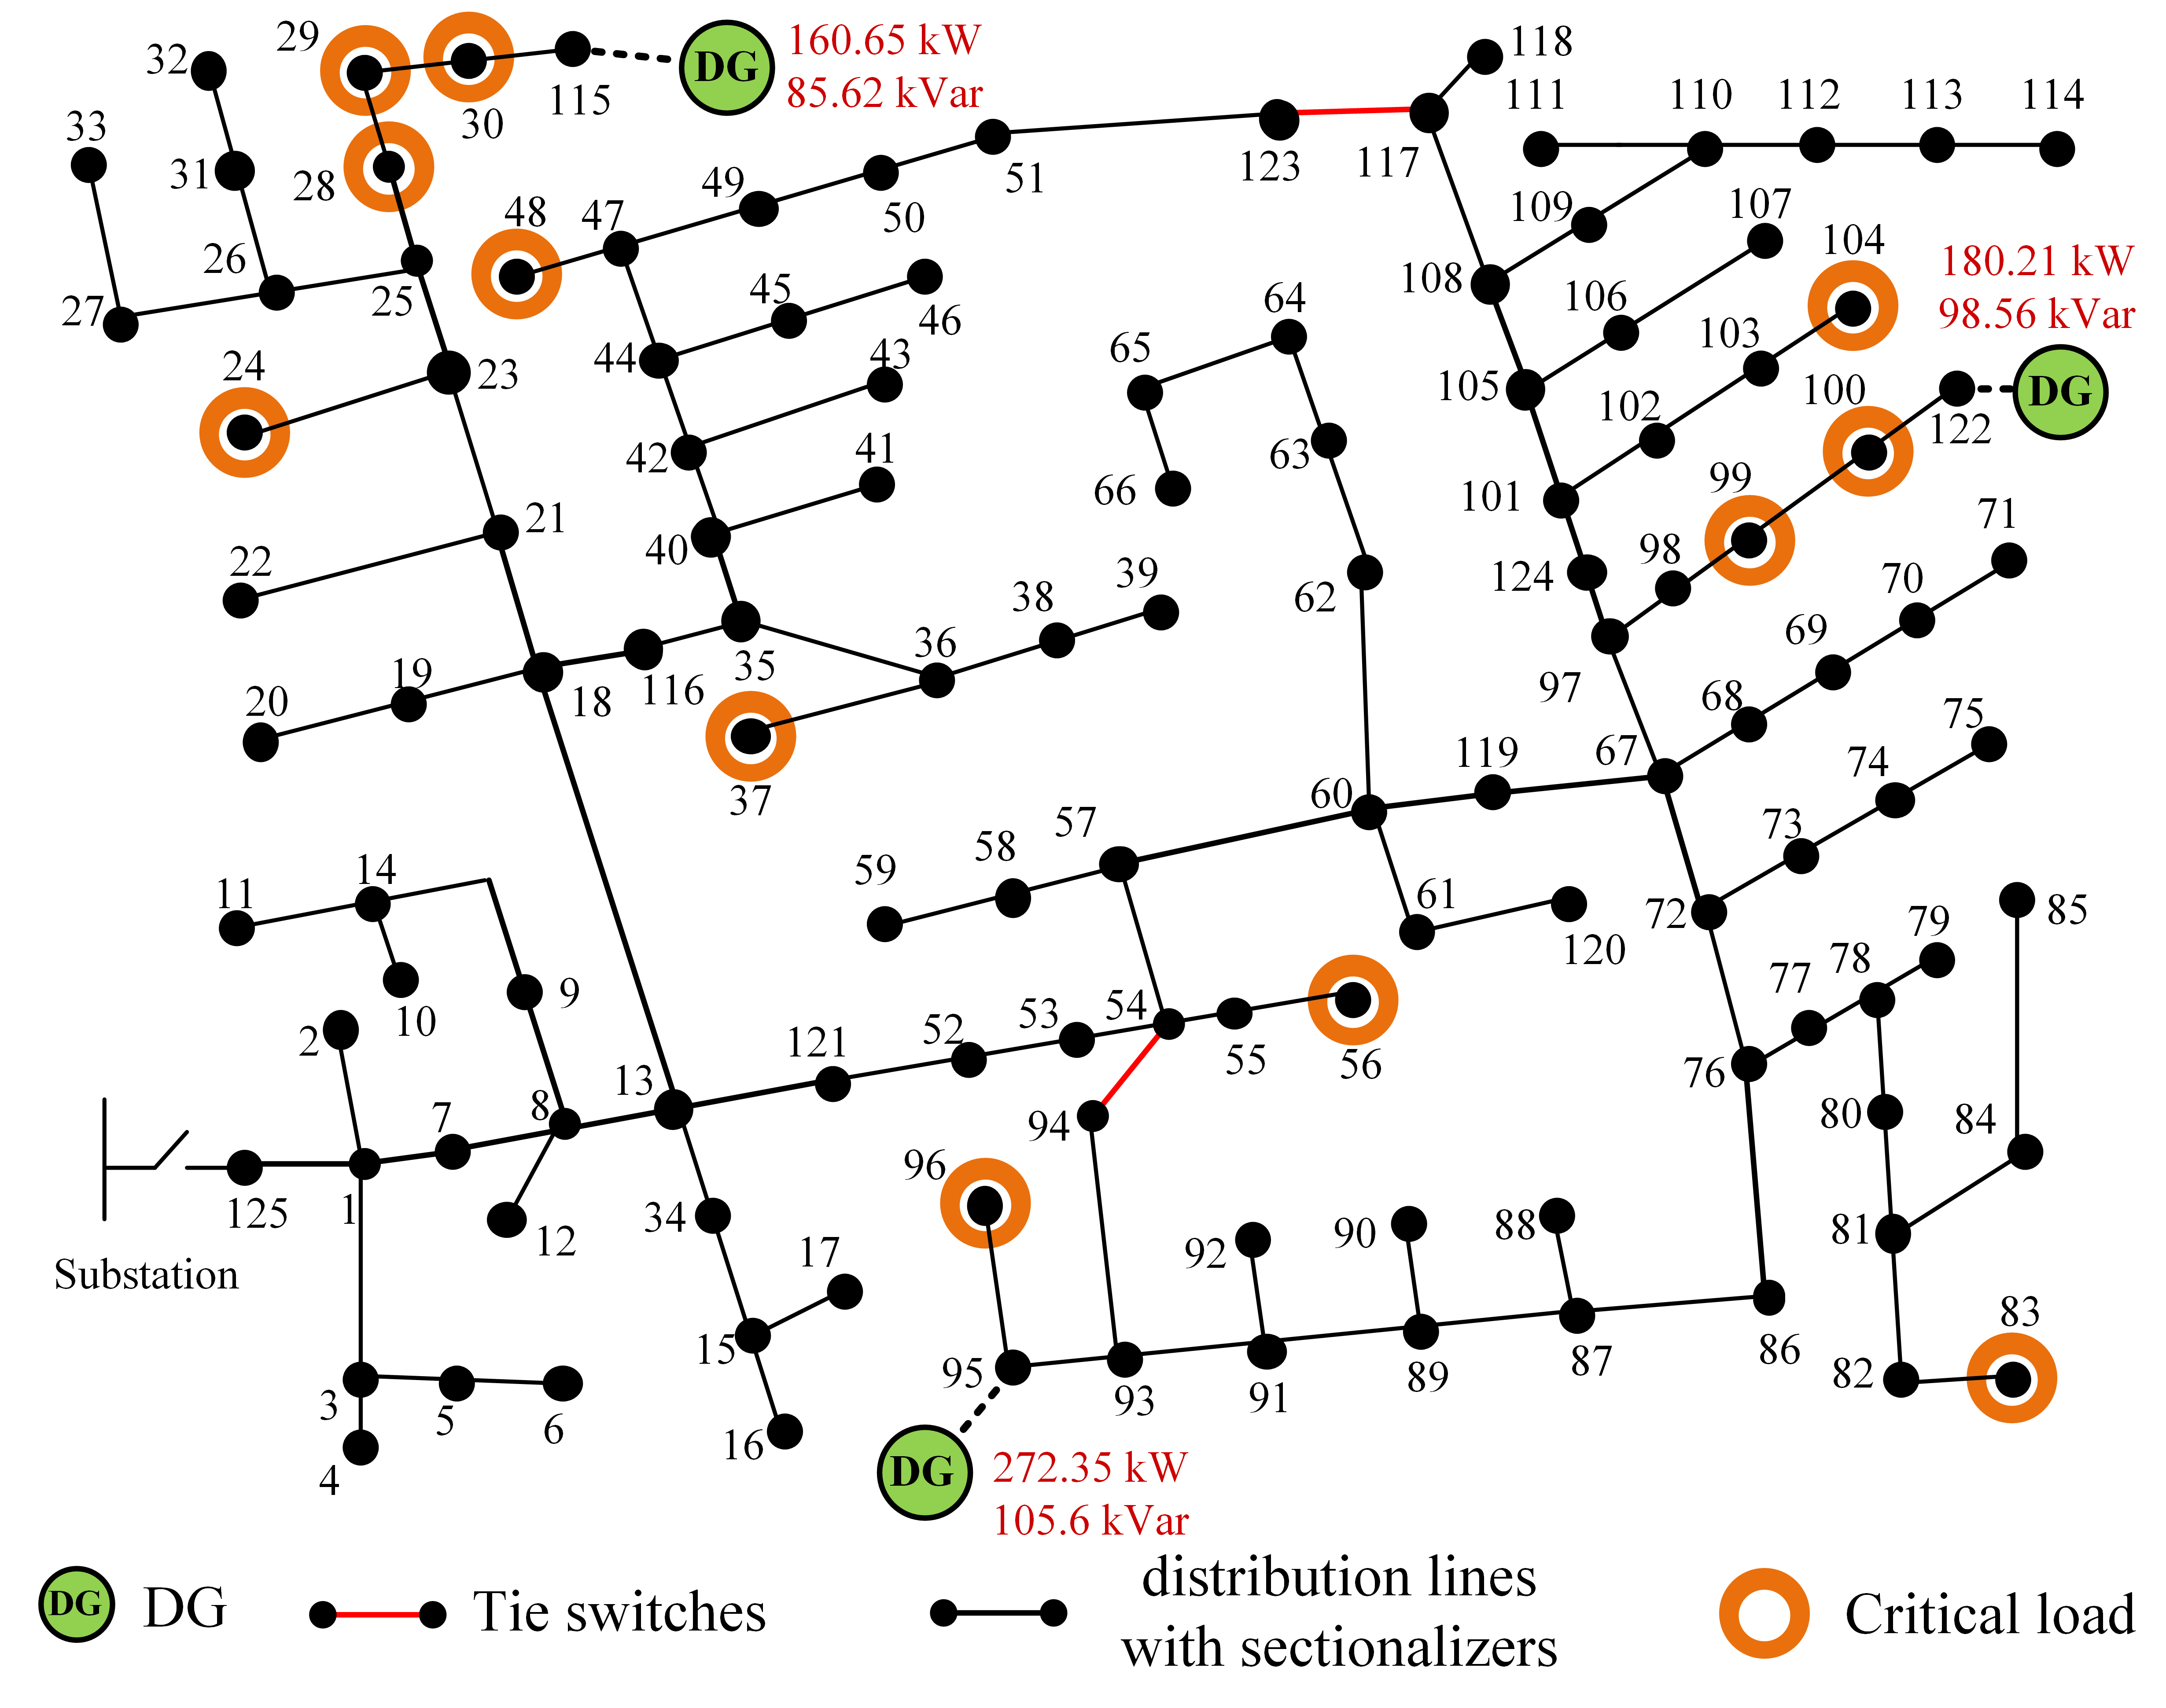
\includegraphics[width=0.55\textwidth]{figures/IEEE_123_testcase.png}
    \caption{Modified IEEE-123 test case with DGs, tie switches, and CLs.}
    \label{fig:IEEE_123_testcase}
\end{figure}

\paragraph{Calculating CVaR of Parameters:}
The five parameters defined in Section~\ref{par:resilience_parameter} are calculated based on Fig.~\ref{fig:resilience_curve} and using the simulation method described above. Fig.~\ref{fig:availability} shows the PDF of $\mathcal{R}_\psi$ obtained for each wind speed along with $VaR_\alpha$ and $CVaR_\alpha$ values. For all of the cases, the value of $\alpha$ is set to be 0.95. The $VaR_\alpha$ and the $CVaR_\alpha$ are calculated using~(\ref{eq:var}) and~(\ref{eq:cvar}). The risk metrics for other parameters are calculated in a similar fashion and are shown in Table~\ref{tab:CVAR}. Each of the parameters are normalized using min-max normalization technique for generality.  

\begin{figure}
    \centering
    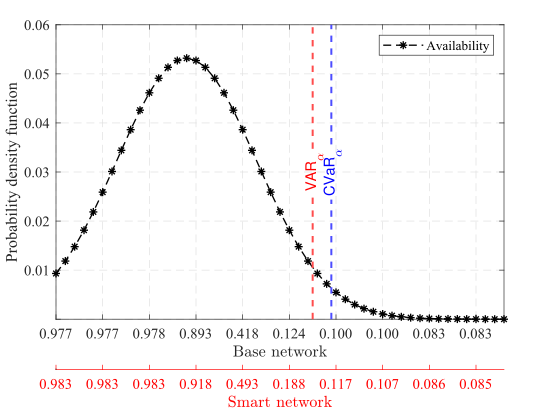
\includegraphics[trim=0cm 0.3cm 1.45cm 0.5cm,clip,width=0.55\textwidth]{figures/Availability.png}
    \vspace{-5pt}
    \caption{PDF of availability for base and smart network.}
    \label{fig:availability}
\end{figure}


%%%%%%%%%%%%%%%%% table for CVaR values %%%%%%%%%%%%%%%%%%%%%
\begin{table}[h]
    \centering
    \caption{$CVaR_\alpha$ of normalized resilience-based \\ parameters for base and smart network}
    \begin{tabular}{c|c|c|c|c|c}
    \hline
          Cases & $\mathcal{R}_\psi$ & $\mathcal{R}_\beta$ & $\mathcal{R}_\gamma$ & $\mathcal{R}_\xi$ & $\mathcal{R}_\delta$  \\
    \hhline{======}
         Base & 0.01115 & 0.00012 & 0.01656 & 0.0037 & 0.00005 \\
    \hline
         Smart & 0.01932 & 0.00012 & 0.01656 & 0.0039 & 0.00314 \\ 
    \hline
    \end{tabular}
    \label{tab:CVAR}
\end{table}



\paragraph{Quantifying Resilience using Choquet Integral:}
To compute the resilience metric based on the multiple parameters and their respective importance, five different cases are developed. For each of the cases, $\mu(.)$ is assigned for each parameter as shown in Table~\ref{tab:weights}. These are the initial fuzzy weights given by the experts or system operators that indicate the priority of one parameter over others.   


%%%%%%%%%%%%%%%%% table for initial weights %%%%%%%%%%%%%%%%%%%%%
\begin{table}[h]
    \centering
    \caption{Initial fuzzy weights of parameters \\ for resilience metric calculation}
    \begin{tabular}{c|c|c|c|c|c}
    \hline
          Cases & $\mu(\mathcal{R}_\psi)$ & $\mu(\mathcal{R}_\beta)$ & $\mu(\mathcal{R}_\gamma)$ & $\mu(\mathcal{R}_\xi)$ & $\mu(\mathcal{R}_\delta)$  \\
    \hhline{======}
        I & 0.9 & 0.25 & 0.15 & 0.6 & 0.85 \\
    \hline
        II & 0.6 & 0.5 & 0.45 & 0.5 & 0.6 \\ 
    \hline
        III & 0.3 & 0.8 & 0.85 & 0.6 & 0.2 \\ 
    \hline
        IV & 0.9 & 0.6 & 0.6 & 0.6 & 0.2 \\ 
    \hline
        V & 0.2 & 0.6 & 0.6 & 0.6 & 0.9 \\ 
    \hline
    \end{tabular}
    \label{tab:weights}
\end{table}

Table~\ref{tab:shapely} shows the Shapely value of each of the parameters as obtained from their initial fuzzy weights. These values also indicate the marginal contribution of each of the parameters in the respective cases. For instance, in Case I the importance of $\mathcal{R}_\psi$ and $\mathcal{R}_\delta$ are greater than the importance of other parameters. Hence, these two parameters contribute more towards resilience quantification than the others. For different cases, the marginal contribution of each of the parameters differ according to the priority set by the system operator or expert.


%%%%%%%%%%%%%%%%% table for Shapely values %%%%%%%%%%%%%%%%%%%%%
\begin{table}[h]
    \centering
    \caption{Shapely values of each parameters \\ based of their initial weights.}
    \begin{tabular}{c|c|c|c|c|c}
    \hline
          Cases & $\eta_{\mathcal{R}_\psi}$ & $\eta_{\mathcal{R}_\beta}$ & $\eta_{\mathcal{R}_\gamma}$ & $\eta_{\mathcal{R}_\xi}$ & $\eta_{\mathcal{R}_\delta}$  \\
    \hhline{======}
         I & 0.35235 & 0.07617 & 0.04451 & 0.20400 & 0.32294 \\
    \hline
         II & 0.23225 & 0.18573 & 0.16404 & 0.18573 & 0.23225 \\ 
    \hline
         III & 0.09441 & 0.30385 & 0.33202 & 0.20849 & 0.06121 \\ 
    \hline
         IV & 0.34422 & 0.19903 & 0.19903 & 0.19903 & 0.05869 \\ 
    \hline
         V & 0.05869 & 0.19903 & 0.19903 & 0.19903 & 0.34422\\
    \hline
    \end{tabular}
    \label{tab:shapely}
\end{table}

%%%%%%%%%%%%%%%%% table for Choquet Integral %%%%%%%%%%%%%%%%%%%%%
\begin{table}[h]
    \centering
    \caption{Choquet Integral values based on \\ Shapely values of each parameters}
    \begin{tabular}{c|c|c|c|c|c}
        Network & Case I    &   Case II   & Case III & Case IV & Case V  \\
    \hhline{======}
        Base  & 5.45 & 6.03 & 7.36 & \textbf{7.89} & 4.72 \\
    \hline
        Smart & 9.36 & 8.68 & 8.36 & \textbf{10.93} & 6.31 \\ 
    \hline
    \end{tabular}
    \label{tab:CI_resilience}
\end{table}

The Choquet Integral values for the base and the smart network and each of the cases are shown in Table~\ref{tab:CI_resilience}. It can be seen that the resilience of the smart network is always greater than that of the base network regardless of individual test cases due to the presence of DGs. However, the resilience for individual networks varies with the Shapely values of each of the parameters. For instance, if we look at the smart network, Case IV is more resilient than any of the other cases as higher priority is given to load availability and infrastructural investments (i.e., $\mathcal{R}_\beta$, $\mathcal{R}_\gamma$, and $\mathcal{R}_\xi$). However, this is not true for the base network as loads are not picked up during the restoration phase in the base network making its availability lower than the smart network. It is also interesting to notice that, the resilience for Case I and Case IV does not have a huge difference although for Case I, the priority towards infrastructural investment is less. Hence, the operators can have the flexibility to focus more on less expensive decisions and still enhance the system's resilience.       


%%%%%%%%%%%%%%%%%%%%%%%%% NEXT CHAPTER %%%%%%%%%%%%%%%%%%%%%
\newpage
\subsection{Risk-based Resilience Planning of Power Distribution Systems}
\subsubsection{Prior work on Power Distribution Planning and their limitations}
The existing literature on power distribution resilience includes numerous articles on operational planning to mitigate or reduce the impact of an imminent threat such as an upcoming storm~\cite{8409997}. Such solutions build resilience via operational response rather than infrastructural upgrades. In operational planning, the decisions are to be made for an upcoming event that is known with a high level of certainty and thus requires considering only a limited number of scenarios for decision-making. On the contrary, long-term planning requires a probabilistic analysis over a wider range of scenarios with a higher level of uncertainty for decisions related to system hardening, infrastructure upgrades, resource allocation, and sizing ~\cite{7381672}. These decisions must also connect to the operational problem if and when the events are realized in practice. Thus, the problem is further complicated by additional stages of operational decision-making leading to an explosion of state space to be considered for decision-making. 

The related literature on resilience-oriented design and pre-disaster resource allocation usually employ a stochastic programming model to minimize the expected cost of the future operational scenarios  \cite{gao2017resilience , zhang2021stochastic}. For example, in \cite{gao2017resilience}, a heuristic search is employed to identify the optimal restoration path and obtain a resource allocation plan. These solutions, however, consider short-term operational requirements for a known HILP event and are not suitable for infrastructure planning. The related work on resilience-oriented distribution system long-term planning also employs stochastic optimization formulations, including a tri-level robust optimization model \cite{yuan2016robust, wang2018resilience}, and a two-stage stochastic optimization model \cite{ma2018resilience, ma2019resilience, liu2019unified}. The tri-level optimization model formulates the resulting problem in a defender-attacker-defender model that is then converted into an equivalent bi-level model and solved using iterative approaches such as CCG or greedy search algorithms~\cite{yuan2016robust}. The tri-level approach optimizes for the worst possible outcomes and hence is not suitable for a probabilistic analysis for infrastructure planning that needs to be cost-effective and optimal for a large range of future scenarios. Alternatively, the two-stage stochastic programming method considers the overall impact of stochastic fault scenarios in planning decisions rather than just the worst-case scenarios \cite{ma2018resilience, shi2020resilience}. The existing two-stage stochastic optimization formulations used in resilience-oriented distribution grid design either assume that all scenarios are observed with equal probability or perform the planning based on only a targeted set of scenarios~\cite{2021IASTATE, 8329529, 9136725}. While such methods are generally applicable, other approaches such as importance sampling and stratified sampling techniques can be more effective in representing HILP events and their impact probabilities in the optimization process~\cite{glynn1989importance, rush2000stratified}. These techniques are widely adopted in power systems reliability studies~\cite{8887536, 7084698}. For a resilience-oriented long-term planning problem, the goal is to determine optimal investments to reduce the consequences (here, customer outages) of the HILP events. Mathematically, this amounts to minimizing the mean of consequences and, more importantly, reducing the tail of the consequence of the HILP events~\cite{9120304}.
